\chapter{Introduction}
\label{Chapter1}
\section{Background and Motivation}

% Lasso -> Bayesian Lasso -> Bayesian Lasso Problem -> challenges of Bayesian Lasso -> % Approximate Bayesian Inference(refer to bayesian paradigm) -> Variational Inference -> % motivation

%%%%%%%%%%%%%%%% Next Version
%%%%%%%%%%%%%%%%

%\textbf{Why Bayesian Lasso problem}
%Advantages: 1. Incorporate Variation (inferential quantity), bring prior if we haev strong prior , %2. Bayesian: Potential for auotomatic tuning selection while Freq cross validation)
%Disadvantages:
%Lasso -> bayesian lasso -> MCMC approximate bayesian inference

\textbf{Introduction of Lasso Problem}\\
The Least Absolute Selection and Shrinkage Operator(Lasso) regression proposed by \cite{tibshirani_1996} belongs to one of the shrinkage methods. As one of the most traditional shrinkage methods, Lasso regression has been proven for his success in Statistical Community over the years.

The Lasso serves as two purposes, one is the estimation of regression parameter, the other is to effective shrinking of the coefficients to achieve variable selection purpose, which is also the fundamental difference of Lasso with other methods. The Lasso Regression is helpful particularly for high-dimensional data because of its sparsity nature.

\textbf{Explain purpose of Lasso}
The definition of linear regression model of interest can be referred based on the following definition defined by \cite{tibshirani_1996}: the $n \times 1$ vector of regression coefficient $\beta$,  $y$ is the response variable with a dimension of $n \time 1$, $X$ is data matrix after standardization with a dimension of $n \times p$ , $\mu$ is the population mean with a dimension of $n \times 1$, $\epsilon$ is independent and identically distributed normal noise with expectation of 0 and variance of $\sigma^2$. Then the linear model can be explained by the Equation \ref{eq:LRmodel}
\begin{equation}
	\label{eq:LRmodel}
	y = \mu 1_n + X\beta + \epsilon.
\end{equation} 
The Least square estimator suggest the sum of square of the difference between estimated response variable and true response variable should be used as loss function as described in Equation (\ref{eq:OLS})
\begin{equation}
	\label{eq:OLS}
	\hat{\beta} = \underset{\beta}{\operatorname{argmin}}  (\tilde{y} - X\beta)^T(\tilde{y}-X\beta).
\end{equation}
 The Lasso estimate of regression coefficient is based on Equation (\ref{eq:lasso1}), where the main distinction of Lasso is adding a penalty term of absolute value of regression coefficients $\beta$ in addition to the sum of squared value of residuals from ordinary regression objective function. The value of tuning parameter $\lambda$ is served as a measure of the extent of penalization.
 \begin{equation}
 	\label{eq:lasso1}
 	\hat{\beta}_{lasso} = \underset{\beta}{\operatorname{argmin}} (\tilde{y}-X\beta)^T(\tilde{y}-X\beta) + \lambda ||\beta||_1, \lambda \geq 0. \tilde{y} =  y - \bar{y}\textbf{1}_n \\
 \end{equation}
 Larger penalization leads to more sparse solution of regression coefficient due to a square constraint set results from $L_1$ penalty function, so that achieve variable selection of parameter, generating a higher prediction accuracy as well as interpretable model since we could drop the estimated regression coefficient that has 0 and state they have weak effect for prediction according to \cite{tibshirani_1996}.
However, due to non-existence of derivative of absolute value of regression coefficient $\beta$, alternative improved algorithm have been purposed and deployed such as Least Angle Regression(LARS), iterative soft-thresholding, subgradient method, and iteratively reweighted least square(IRLS) by \cite{efron_hastie_johnstone_tibshirani_2004},   \cite{beck_teboulle_2009}, \cite{nan_zhang_shuqing_zeng_2005} and \cite{friedman_hastie_tibshirani_2010}.

\textbf{Bayesian Lasso}
One of the detriments of the ordinary lasso is that the variation of inferential quantity can't be captured properly. To resolve this issue, \cite{tibshirani_1996} also suggests that the lasso estimate can also be extended under the Bayesian framework, which can be described as posterior mode Equation(\ref{eq:MLELasso}) if independent and identically distributed Laplacian prior from Equation (\ref{eq:LassoPrior}) is assigned,together with the likelihood form on Equation(\ref{eq:lassolikelihood}). 
\begin{equation}
	\label{eq:MLELasso}
	\hat{\beta}_{lasso} = \underset{\beta}{\operatorname{argmax}}P(\beta|y,\sigma^2,\tau), \tau = \frac{\lambda}{2\sigma^2}
\end{equation}
\begin{equation}
	\label{eq:LassoPrior}
	f(\beta_j) = (\frac{\tau}{2})^p exp(-\tau|\beta_j|),
\end{equation}
\begin{equation}
	\label{eq:lassolikelihood}
	p(y |\beta,\sigma^2) = N(y|X\beta,\sigma^2I_n).
\end{equation}
% Add full models
\textbf{Introduction of Bayesian Lasso Problem(Why Bayesian Lasso)}
Nevertheless, there is no tractable integration form for the Bayesian Lasso posterior until \cite{park_casella_2008} further explore the Lasso model under the setting of Bayesian framework, where the choice of a conditional Laplace prior distribution over the regression coefficient $\beta$ conditioning by standard error $\sigma^2$ is added to the Lasso penalty formulation in the frequentist framework to ensure unimodality of full posterior distribution. Based on closed form of tractable posterior distribution, a three-step Gibbs sampler is proposed to draw approximate samples from Bayes Lasso posterior distribution, which can be utilized for further inference of parameter of interest.
\begin{equation}
	\label{eq:lassoprior}
	\pi(\beta |\sigma^2) = \prod_{j=1}^p \frac{\lambda}{2\sqrt{\sigma^2}} e^{-\lambda|\beta_j|/\sqrt{\sigma^2}}
\end{equation}
There are several benefits for using the Bayesian Lasso model. Firstly, it has easier implementation than the traditional Lasso, although more computation of conditional distribution form is demanded. Secondly Bayesian credible interval of parameters can be generated simultaneously for modelling uncertainty and therefore can also guide variable selection based on the interpretation that lasso estimated is regarded as the mode of posterior distribution of $\beta$. 
Thirdly, \cite{park_casella_2008} also state that the Bayesian Lasso model could also be a potential solution for addressing the issue of attaining optimal tuning parameter $\lambda$ by marginal maximum likelihood method together with a sue of an suitable hyperprior such as gamma prior on the square of tuning parameter $\lambda$: $\lambda^2$. 
It could support a more stable automatic tuning process of choosing the most appropriate tuning parameter $\lambda$ for the Lasso problem, as opposed to inefficient $K$-fold cross validation approach under the ordinary Lasso model that is time consuming and computational demanding. Lastly, the three-step Bayesian Lasso Gibbs Sampler proposed by \cite{park_casella_2008} would yield an exact posterior distribution that can be sampled given exact form of conditional distribution of each model parameter conditioning on rest of the other parameters. Theoretically, \cite{khare_hobert_2013} has demonstrated a Bayesian Lasso Gibbs sampler version of central limit theorem(CLT), indicating Bayesian Lasso Gibbs Sampler satisfy geometriclly ergodicity if any values of sample size $n \geq 3$ and arbitary number of regression coefficient $p$, data matrix $X$, tuning parameter $\lambda$ are assigned. This means, the Bayesian lasso Gibbs Sampler is able to achieve asymptotically uncertainty of posterior estimation. To address this issue, \cite{FastBL} invented a reduced step Gibbs sampler instead, successfully accelerating the sampling procedure. 


\textbf{Approxiamte Bayesian Inference Intuition}

Review of Bayesian inference intuition can be referred from Section \ref{bayeisanP}, but challenges of Bayesian Inference motivates the approximate bayesian inference method thereafter. To be specific, \cite{bishop_2006} states three main challenges of obtaining posterior distribution. Firstly, the dimension of target parameter might be high, which results in heavy computational cost for estimating posterior distribution. Secondly, the exact posterior distribution form might be too complicated to be tractable,. Thirdly, the computation of the posterior mean parameter $\int_{\theta} \theta p(\theta|\mathcal{D})$ has high probability without having an simple calculation, resulting in the fact that there might not exist an closed form analytical solution for integration. Much efforts have been paid over the years, there are two main types of sampling approach that are effective currently, which are stochastic sampling algorithms and deterministic approximation algorithms. 

\textbf{Introduction of ABI method}
There are two genres of Approximate Bayesian Inference method, which includes stochastic approach such as MCMC, where an exact result can be obtained if infinite computational resource is assigned. Another category lies in deterministic approach that as an faster substitution compared with stochastic approximation approaches.
As stated above, an approximate inference method such as MCMC is used for posterior distribution estimation. The necessity of approximate bayesian inference method is due to its' expensive and infeasible exact posterior distribution parameter estimate.

\begin{equation}
	p(\theta|\mathcal{D}) = \frac{p(\mathcal{D}|\theta)p(\theta)}{p(\mathcal{D})},
	\label{eq:Bayesrule}
\end{equation}

\textbf{Challenges of Bayesian Lasso model}
 Returning back to the Bayesian Lasso model, the three-step Gibbs sampler belongs to the class of MCMC algorithm, which produce samples demonstrates gradually decreasing correlated samples as the burn-in period is increased. Burn-in period refers to the time the sample before that period have to be abandoned. On the other hand, the three-step Gibbs sampler from Markov Chain Monte Carlo(MCMC) under the class of stochastic approximation algorithm is time-consuming and computational challenging, given the fact that it normally requires a long time to converge inside the interval of an acceptable tolerance, especially when $n$ is small and $p$ is large derivation according to the upper bound of convergence rate by \cite{rajaratnam_sparks_2015}. 


\textbf{Approximation Algorithm: Deterministic type \& VI}.
 Due to limitation of stochastic type of algorithm, alternative methods such as deterministic Variational Inference methods has becoming popular due to its fast speed and simple computation. 
 Numerous algorithms have been designed and utilized widely such as Variational Bayes, Expectation Propagation algorithms etc. A common variation is Coordinate Ascent Variational Inference approach produced by \cite{Blei2003LDA} , which assume the approximation originates from a analytically tractable class of distribution $Q$ first and attempt to search for the distribution from this family that is the closest to the target posterior distribution with some discrepancy metric such as the Kullback–Leibler divergence etc.  
 An optimization based system in Equation (\ref{eq:VI1}) is established by iteratively updating variational parameter with an appropriate optimization algorithm such as Coordinate Ascent to obtain approximated posterior distribution that is in the family of $Q$, while the most common choice is the Normal Distribution due to its simple form and adaptability to other distribution.
 To further illustrate the intuition, Figure \ref{fig:VIoptimization} provides further explanation of aforementioned intuition, goal and procedure of Variational Inference.
 
 \begin{figure}[H]
 	\center
 	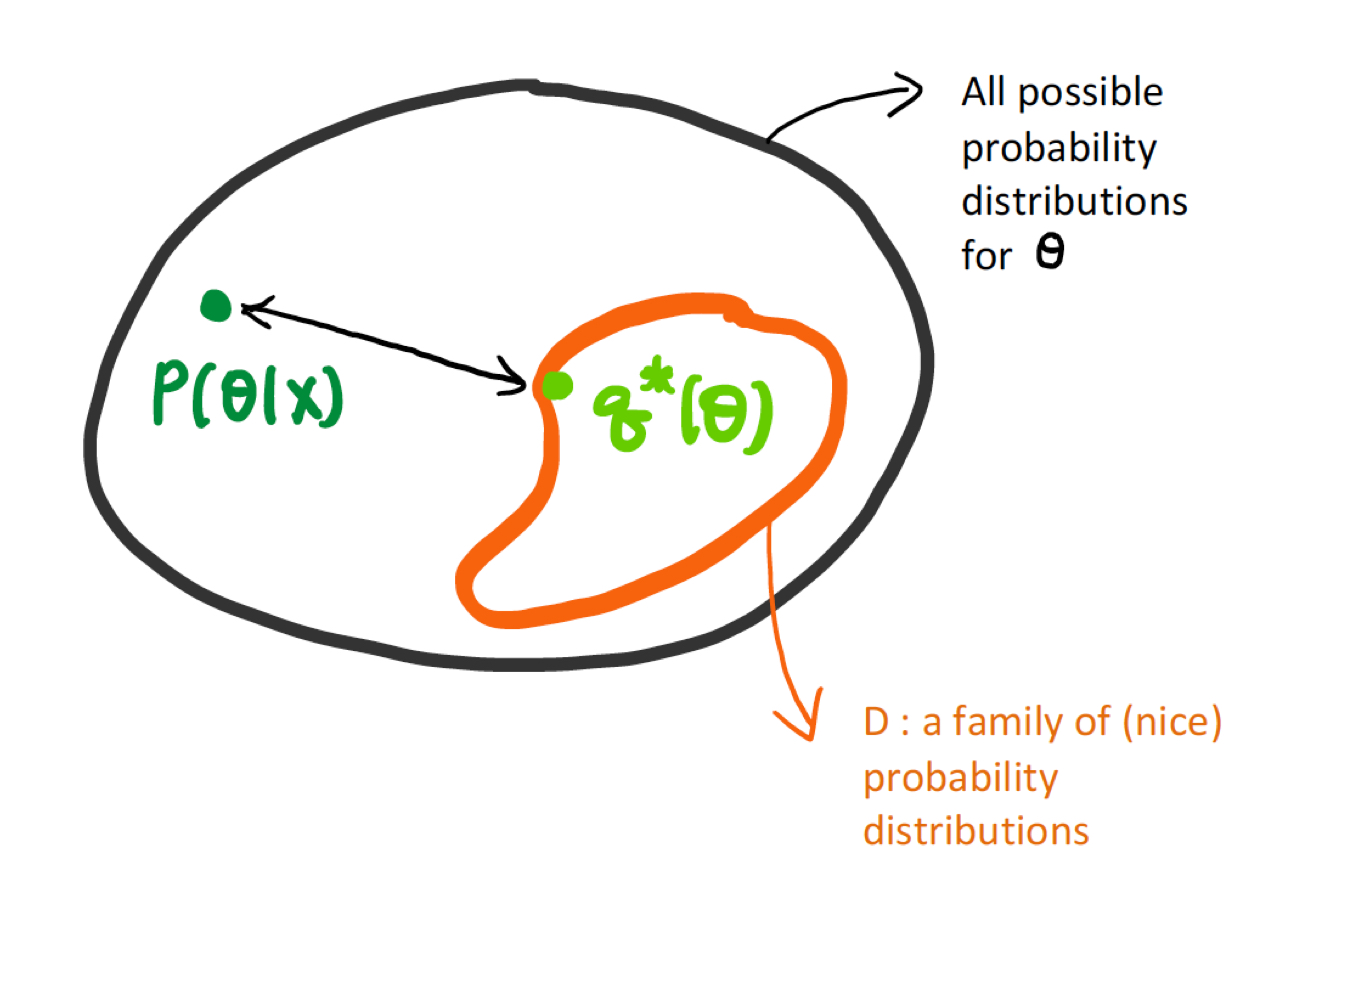
\includegraphics[scale = 0.2]{VIoptimization}
 	\caption{Variational Inference intuition, where $X$ is data $\mathcal{D}$, $D$ is equivalent to $Q$ defined above}
 	\label{fig:VIoptimization}
 \end{figure}

\begin{equation}
	\label{eq:VI1}
	q^{*}(\theta) = \underset{q_{\theta} \in Q}{\operatorname{argmin}} \textnormal{KL}(q(\theta)||p(\theta|\mathcal{D})) \coloneqq \int q(\theta)\log(\frac{q(\theta)}{p(\theta|\mathcal{D})})d\theta
\end{equation}

\begin{equation}
	\label{eq:KL2}
	\textnormal{KL}(q||p(.|\mathcal{D})) = - \int q(\theta)log(\frac{p(\theta)p(\mathcal{D}|\theta)}{q(\theta)}) d\theta + \log p(\mathcal{D}).
\end{equation}
In addition, the exact form of $\textnormal{KL}$ divergence can be found in Equation (\ref{eq:KL2})
In practice, the minimization of $\textnormal{KL}$ divergence from Equation (\ref{eq:VI1}) would be converted into an equivalent formulation in Equation (\ref{eq:KL}) that maximize the lower bound of $\log(p(y))$ due to complexity of minizing the original $\textnormal{KL}$ divergence, which can also be called Evidence Lower Bound(ELBO) that can be defined by by Equation (\ref{eq:KL}).
\begin{equation}
	\label{eq:KL}
	q^*(\theta) = \underset{q_{\theta} \in Q}{\operatorname{ argmax}} \textnormal{ELBO}(q(\theta)),
\end{equation}
\begin{equation}
	\label{eq:ELBO}
	\textnormal{ELBO}(q(\theta)) = \int q(\theta)\log(\frac{p(\theta)p(\mathcal{D}|\theta)}{q(\theta)} = \mathop{\mathbb{E}_{q(\theta)}}\log(\frac{p(\theta)p(\mathcal{D}|\theta)}{q(\theta)}).
\end{equation}

\textbf{Mean Field Variational Bayes, History and introduction}
The most traditional Variational Inference algorithm is known as Mean-Field Variational Bayes motivated by mean-field Theory in statistical physics yielded by 
\cite{jordan_ghahramani_jaakkola_saul_1998} and \cite{attias_1999}, which assume the approximated distribution is from independent product of parameter distribution from set $Q$ as in Equation (\ref{eq:MFVBassume}) if assuming there are $k$ sub-parameter of target parameter $\theta$.
\begin{equation}
	\label{eq:MFVBassume}
	q(\theta) = \prod_{i=1}^{k} q_i(\theta)
\end{equation}
Mean-Field Variational Bayes have been adapted and developed over the next two decades, especially in mixture modelling and probabilistic graphical model. It sometimes provide efficient variable selection as well, We will introduce more about the algebra of MFVB in Chapter \ref{Chapter2}. Variational Inference community benefits from MFVB due to its tractable family of 

\textbf{Advantages of Variational Inference}
Variational approach is more superior and appropriate at present for several reasons according to \cite{blei_kucukelbir_mcauliffe_2017}. One is that Variational Inference algorithm shows a descent computation cost and scalability, and thus Variational inference can be adaptive when the amount of data is huge. For instance, if there exists a billion image that requires to be fitted into probabilistic machine learning model, then exact precision method such as MCMC will be computataional demanding, while Variational Inference would sacrifice tiny accuracy with hundreds of time faster speed as return.
%Another important factor is that distributed computation and stochastic optimization technique can be embedded to the Variational Inference framework due to its nature of an optimization system, while the Variational Inference originates from Machine Learning for approximating probability density for complex probabilistic graphical model \cite{jordan_ghahramani_jaakkola_saul_1999}. 
Secondly, the descent time-efficiency of Variational Inference becomes another significant factor why it is popular, given the fact it only involves updating variational parameters iteratively until convergence, as opposed to MCMC that produce correlated samples that limit the ideal behavior of MCMC algorithm.

\textbf{Drawbacks of VI}
Meanwhile, disadvantages of Variational Bayes include inexact approximation result under some scenarios, although it could capture marginal density. For example, it is suggested by \cite{blei_kucukelbir_mcauliffe_2017},
%Might have problem with citation pRML%
that Variational Inference algorithm might underestimate the covariance between parameter of interest, if inter-parameter correlation is strong. It tends to ignore the correlation between parameters, results in unideal behavior as a resullt. Figure \ref{fig:VIdemo}
further demonstrates this phenomenon, the ture overall posterior of $x_2$ and $x_1$ have a exploded correlation with a eclipse-shaped density, while a circled-shape mean-field approximation is established instead due to its product density family limitation.
\begin{figure}
	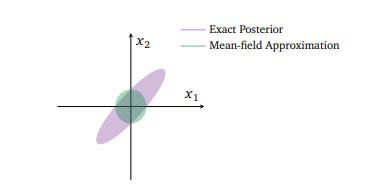
\includegraphics[width=\linewidth]{VIdemo}
	\caption{Visualization of Mean-Field Variational Approximation compared with exact posterior when correlation is large}
	\label{fig:VIdemo}
\end{figure}
We will expand properties and derivation of Variational Inference more in subsection \ref{VI}.

Overall, Variational Inference has proven its effectiveness in distinct application fields such as speech recognition and document retrieval in natural language processing, computer vision etc. Despite small disadvantages of Variational Inference, the potential of variational approximation haven't been fully discovered yet by researchers, its ability to provide reliable posterior estimate is invaluable in the future in the era of big data and deep learning nowadays.

\textbf{Motivation}
Motivated by the intention of further enhancing the approximation accuracy of Variational Bayes, as well as the oracle property of Bayesian Lasso regression coefficient estimation for variable selection and standard error estimation leads to more desired demand for fast approximate inference. We would like to design new Variational Inference based algorithms for the Bayesian Lasso regression problem, for the purpose of obtaining bayesian lasso posterior distribution in a much faster and more accurate manner based on the Mean-Field Variational Bayes assumption.

Feeding initial value of mean $\mu$ and covariance parameter $\Sigma$ and writing out the marginal likelihood form of regression coefficient $\beta_i$ for $j$ th variable, $\log(p(\mathcal{D})|\beta_j)$, we've invented a new distribution called univariate lasso distribution for matching the marginal likelihood. Mixing each marginal likelihood with a Gaussian Approximation, we've shown its' approximation accuracy have surpassed every existing algorithm such as Mean-Field Variational Bayes. Even though the speed of our algorithm is slightly slower than MFVB, the approximation accuracy illustrates a tiny gap between exact estimation from MCMC, with hundred times faster time complexity.
Nevertheless, there is a drawback of this method, given the fact that the global covariance matrix would remain diagonal if the initial global covariance matrix is diagonal.
To remedy this issue, we've also purposed another algorithm based on marginal likelihood estimation by a bivariate lasso distribution. Instead of updating corresponding mean, covariance matrix for each variable for each iteration, the marginal likelihood of each pair of variables would be matched, so that further generalize our algorithm. Our conclusion are the univariate lasso algorithm would be faster with a lower accuracy while bivariate lasso algorithm would be slower with a higher accuracy, since it updates each pair of variables at a time resulting in ${p\choose 2}$ of unique parirs. We will show the full intuition and idea later in Chapter \ref{Chapter3}.
By utilizing and fitting a both univariate and multivariate Lasso distribution to marginal distribution, an improved estimate for global Gaussian Approximation can be obtained as defined in Equation (\ref{eq:GV}). Finally, we will show our experiment result in \ref{Chapter4} using various accuracy metrics.

Our contribution have been listed in the following subsection \ref{cont}.
\begin{equation}
	\label{eq:GV}
	q^{*}(\theta) \approx N(\mu^*,\Sigma^*)
\end{equation}

\section{Contribution}
\label{cont}
Our main contribution could be concluded as the following part:
\begin{itemize}
	\item Introduction of Univariate and Multivariate Lasso Distribution
	\item Derivation of properties for Univariate Lasso Distribution, such as the expectation, variance, Cumulative Density Function form etc.
	\item Derivation of properties for Multivariate Lasso Distribution such as the expectation, variance, Cumulative Density Function form etc.
	\item Implementation of Univariate Lasso Distribution and Multivariate Lasso Distribution property in R.
	\item Design of two new Variational Inference approaches based on local approximation by univariate lasso distribution and multivariate lasso distribution respectively.
	\item Conduct of experiment to testify two algorithms under dataset by several evaluation metrics for approximation accuracy such as Hitters dataset etc.
\end{itemize}



\section{Thesis Organization}
This paper will be divided up into 5 chapters. Chapter 1 briefly illustrate the motivation and background of the Lasso problem, Bayesian Lasso Problem, the motivation for Approximate Bayesian Inference, with a specific focus on determinstic  Variational Approximation. Chapter 2 will briefly review and explain the details of the methodlogy in previous work such as the lasso problem, Approximate Bayesian Inference algorithm, MCMC(Monte Carlo Method), Bayesian Expectation Maximization algorithm and their variants and Mean-Field Variational Bayes(MFVB). We will present our main methodology of variational algorithm in Chapter 3, followed by a comprehensive experiment for testing the effectiveness of algorithm in Chapter 4. 



 